\begin{frame}{Support Vector Machines (SVM)}
Very famous supervised learning algorithm:
\begin{itemize}
\item performs \textbf{binary} classification (can be adapted for multiclass problems)
\item is \textbf{linear} (in its original formulation) 
\item main feature: chooses the decision boundary that \underline{maximizes the margin} between positive and negative examples
\end{itemize}
\begin{columns}
\begin{column}{0.5\textwidth}
\begin{center}
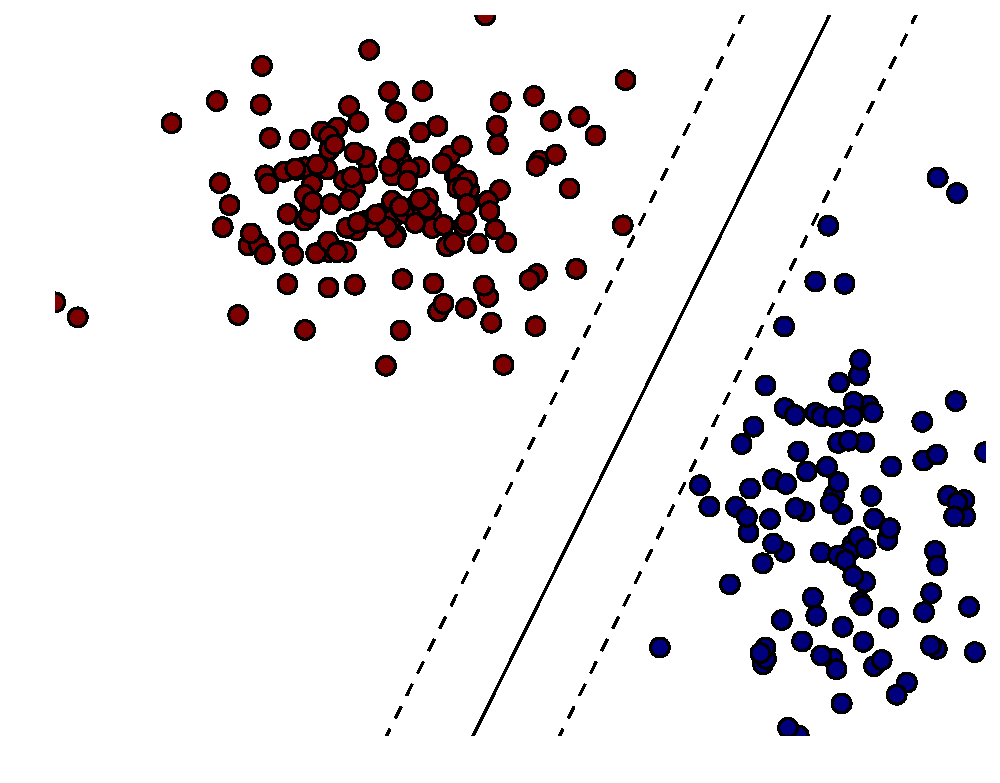
\includegraphics[width=0.7\textwidth]{img/svm/max_margin.pdf}
\end{center}
\end{column}
\begin{column}{0.5\textwidth}
How do you find such line?
\end{column}
\end{columns}
\end{frame}